In this chapter we will do further analyses of the model results with particular
emphasis on the AttentionSegRank architecture due to it's better performance
and explainability. On section one we will discuss the effects of using semantic segmentation
on neural network  training. Section 2 will show the quantitative relationship between
segmentation, attention and the perception quantification. And finally, section 3 we will
analyze the implications of this method on model explainability.

\section{Effect of semantic segmentation on learning}
As was already mentioned on section \ref{sec:training}, adding a fixed segmentator to
the neural network architecture resulted in a reduction of performance along with a considerable
reduction of overfitting. The behavior was expected when fully replacing the CNN features,
due to the reduced expressiveness of the segmentation and the lack of finetuning, but
unexpectedly, although it is reduced, this behavior persists when combining the fixed
segmentation with the finetuned ResNet50 through the attention layer. We conclude from this
that restricting the attention weights to the shapes and classes given by the segmentation
has a regularizing effect on learning, reducing the model capacity even when the amount of trainable
weights is maintained.

In the case of the PlacePulse dataset this is not a problem since
all traditional deep models suffer of significant overfitting. It remains an interesting research
question  if these behaviors will transfer to other tasks and datasets.

\begin{figure}[ht]
	\begin{center}
	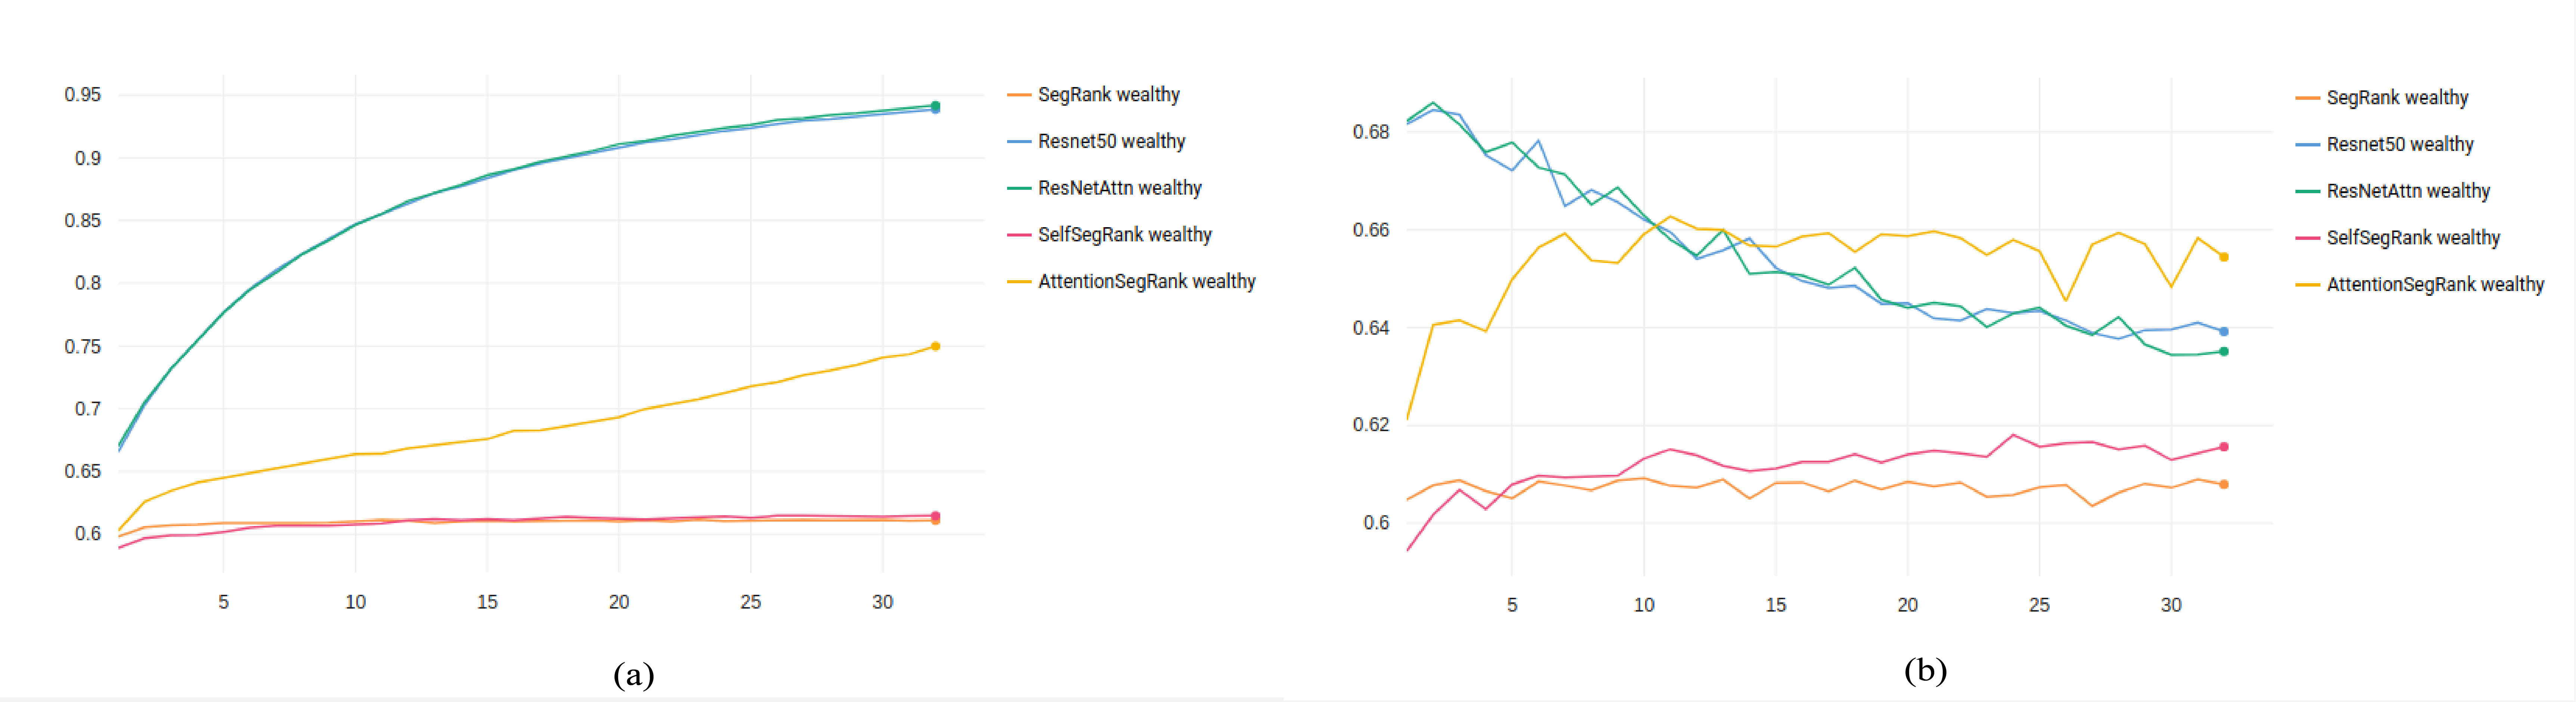
\includegraphics[width=1\textwidth]{./figures/wealthy_graph.png}
	\caption[Wealthy Training curves]{
        Wealthy accuracy vs epoch learning curves on training (a) and validation (b).
        }
	\label{fig:wealthy_graph}
	\end{center}
\end{figure}

\section{Segmentation as an attention subject.}
By combining the outputs of the segmentation and the attention, we can infer if a certain class was
important for the quantification of perception of a single image. We do this by computing the ratio between
the percentage of pixels belonging to a single class and the percentage of attention placed by the model on
those pixels:
\begin{equation}
	\text{significance ratio} = \frac{\% \text{ attention}}{ \% \text{ segmentation}}
\end{equation}

Using that we define that a class is significant in an image when significance ratio $\geq 1$.
Meaning that the total attention received by the pixels belonging to that class is larger
than the amount they would get if the attention was distributed uniformly over the whole image.

We calculate the significance of all the CityScapes classes
on all the images of the validation split for each of the perception attributes. We report
the results on tables \ref{tab:total_sig} and \ref{tab:presence_sig}, which show the percentage
of images where each class is considered significant over the whole split, or filtered by the images
where the class is present respectively.

The most notable insight from this results is that there is considerable differences on the same class
but for different attributes, for example buildings are the most significant for the boring attribute
but is one of the least for the depressing attribute. Vegetation is significant for beautiful and
depressive but not for wealthy. Another insight is that some classes are on average considerably more significant
than others, we believe this happens because they are much more common than others in the dataset
and the networks learn to consider them more often. For the exact distribution of the segmentation classes
see appendix \ref{sec:seg_distribution}.

\begin{table}[H]
	\begin{tabular}{|l|rrrrrrr|}
		\hline
					& \multicolumn{7}{c|}{\textbf{Significance \%}}   \\ \hline
		\textbf{Class}         & \textbf{Wealthy}        & \textbf{Depressing}     & \textbf{Safety}         & \textbf{Boring}         & \textbf{Lively}         & \textbf{Beautiful}      & \textbf{Average}        \\
		\hline
		Road          & 62.46          & \textbf{77.98} & \textbf{78.64} & 31.77          & \textbf{90.58} & 17.33        & \textbf{59.79} \\
		Building      & \textbf{63.74} & 9.21           & 30.35          & \textbf{82.69} & 17.99          & \textbf{52.79} & 42.80          \\
		Sky           & 43.81          & 44.51          & 39.34          & 18.34          & 45.68          & 45.80          & 39.58          \\
		Person        & 4.86           & 18.18          & 10.83          & 28.83          & 25.76          & 6.77           & 15.87          \\
		Car           & 4.09           & 19.70          & 12.02          & 34.63          & 6.12           & 15.50          & 15.34          \\
		Vegetation    & 4.27           & 22.56          & 20.57          & 5.50           & 5.45           & 24.08          & 13.74          \\
		Bicycle       & 4.81           & 8.25           & 10.32          & 15.48          & 16.57          & 10.10          & 10.92          \\
		Sidewalk      & 10.65          & 12.46          & 2.21           & 7.65           & 7.35           & 9.66           & 8.33           \\
		Truck         & 4.65           & 11.38          & 2.94           & 9.57           & 6.29           & 14.29          & 8.19           \\
		Motorcycle    & 4.92           & 5.31           & 6.68           & 8.10           & 9.77           & 10.97          & 7.63           \\
		Wall          & 3.43           & 4.63           & 4.90           & 9.95           & 5.33           & 9.14           & 6.23           \\
		Fence         & 5.33           & 13.15          & 6.83           & 1.75           & 2.17           & 4.55           & 5.63           \\
		Pole          & 1.48           & 2.76           & 2.04           & 8.00           & 13.03          & 3.49           & 5.13           \\
		Terrain       & 0.74           & 2.72           & 2.72           & 13.31          & 1.45           & 4.38           & 4.22           \\
		Traffic sign  & 1.18           & 2.39           & 1.47           & 3.55           & 2.59           & 1.44           & 2.10           \\
		Traffic light & 1.60           & 0.89           & 0.47           & 2.00           & 1.19           & 1.42           & 1.26           \\
		Train         & 0.22           & 1.57           & 0.16           & 0.73           & 0.52           & 3.84           & 1.17           \\
		Bus           & 0.74           & 1.51           & 1.15           & 0.82           & 0.83           & 0.92           & 1.00           \\
		Rider         & 0.49           & 1.12           & 1.02           & 1.10           & 1.23           & 0.98           & 0.99 \\
		\hline
	\end{tabular}
	\caption[Percentage of class significance]{
		Percentage of images where a segmentation class is considered significant over the entire PlacePulse dataset.
	}
	\label{tab:total_sig}
\end{table}

This results support that attention weights are a good way to augment the explainability of
the models since they show that the same architecture learns to attend to different things
when quantifying different attributes.

\begin{table}[H]
	\begin{tabular}{|l|rrrrrrr|}
		\hline
					& \multicolumn{7}{c|}{\textbf{Significance \%}} \\ \hline
		\textbf{Class} & \textbf{Wealthy} & \textbf{Depressing} & \textbf{Safety} & \textbf{Boring} & \textbf{Lively} & \textbf{Beautiful} & \textbf{Average} \\
		\hline
		Sky            & \textbf{78.49}   & \textbf{80.12}      & 70.85           & 33.32           & 82.16           & \textbf{82.62}     & \textbf{71.26}   \\
		Road           & 64.87            & 81.01               & \textbf{81.67}  & 33.06           & \textbf{94.07}  & 18.00              & 62.12            \\
		Rider          & 30.34            & 65.75               & 59.74           & 61.42           & 71.21           & 59.14              & 57.93            \\
		Building       & 69.73            & 10.07               & 33.23           & \textbf{90.59}  & 19.67           & 57.81              & 46.85            \\
		Wall           & 25.11            & 34.35               & 36.34           & 72.00           & 39.70           & 67.03              & 45.75            \\
		Motorcycle     & 23.73            & 25.34               & 32.13           & 38.80           & 46.53           & 51.87              & 36.40            \\
		Bus            & 26.46            & 53.96               & 40.25           & 27.17           & 29.32           & 31.90              & 34.84            \\
		Bicycle        & 14.42            & 24.77               & 30.73           & 45.93           & 49.26           & 30.07              & 32.53            \\
		Person         & 9.61             & 35.91               & 21.37           & 56.87           & 50.77           & 13.35              & 31.31            \\
		Car            & 6.53             & 31.41               & 19.16           & 55.41           & 9.73            & 24.66              & 24.48            \\
		Truck          & 13.13            & 31.95               & 8.26            & 26.92           & 17.51           & 40.09              & 22.98            \\
		Sidewalk       & 28.19            & 33.39               & 5.87            & 20.48           & 19.56           & 25.78              & 22.21            \\
		Traffic sign   & 12.00            & 24.43               & 15.18           & 36.81           & 26.60           & 15.08              & 21.68            \\
		Traffic light  & 26.92            & 15.04               & 8.06            & 34.47           & 20.28           & 24.78              & 21.59            \\
		Train          & 3.96             & 29.40               & 2.95            & 13.57           & 9.38            & 69.82              & 21.52            \\
		Terrain        & 3.35             & 12.39               & 12.40           & 61.04           & 6.63            & 20.23              & 19.34            \\
		Vegetation     & 4.87             & 25.70               & 23.45           & 6.26            & 6.21            & 27.42              & 15.65            \\
		Pole           & 3.89             & 7.19                & 5.35            & 21.04           & 34.17           & 9.15               & 13.46            \\
		Fence          & 10.88            & 26.98               & 14.06           & 3.61            & 4.47            & 9.35               & 11.56            \\
		\hline
	\end{tabular}
	\caption[Percentage of class significance]{
		Percentage of times a segmentation class is considered significant when it is present in an image.
	}
	\label{tab:presence_sig}
\end{table}

We can also visualize which classes are significant for individual examples, allowing
for a simple interpretation of results on a per instance basis.
See figure \ref{fig:ratio} in which the road and sky classes are significant.

\begin{figure}[ht]
	\begin{center}
	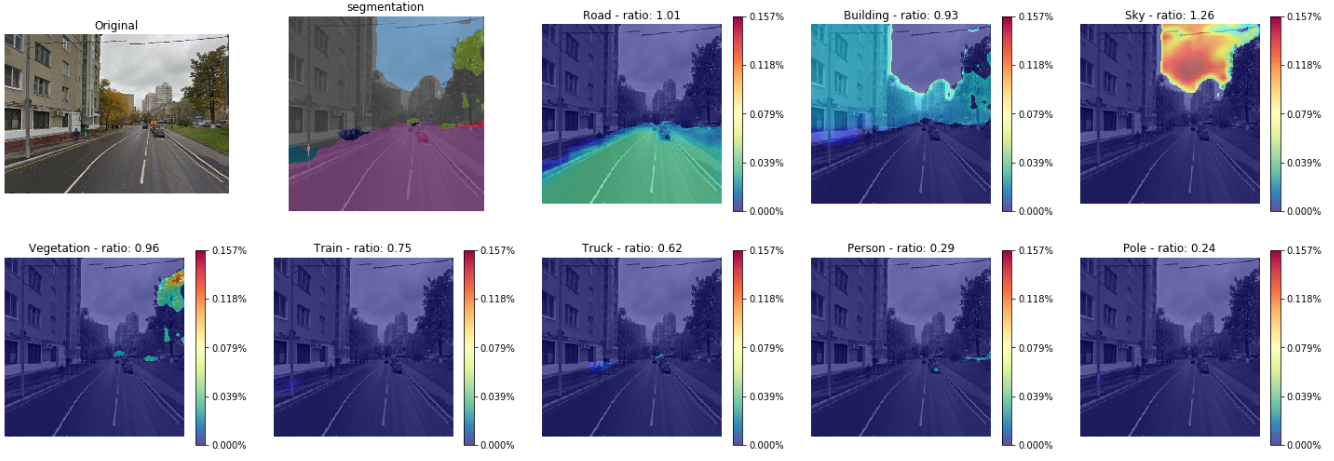
\includegraphics[width=1\textwidth]{./figures/ratio.png}
	\caption[Example of significance ratio]{
        Sample visualization including class significance for the safety attribute.
        }
	\label{fig:ratio}
	\end{center}
\end{figure}


\section{Relationship between urban perception and semantic segmentation}

Similarly to previous work \cite{rossetti, zhang_measuring} we analyze how the segmentation relate with the quantified
perception scores, for that we count the percentage of pixels of each segmentation class
on all the images of the validation split for each of the perception attributes and measure
correlation with the output.

Acá van los graficos del score respecto a la segmentación. y la tabla de correlación

Acá van los comentarios de que cosas son importantes para que atributo y comparamos con rosetti ramirez y zhang.

\section{Effect of attention over semantic segmentation on model explainability}
Acá hablamos de las visualizaciones de atención promedio.

Acá mostramos ejemplos de visualizaciones en que se vean atenciones claras junto con el score.